\documentclass[a4paper,12pt]{article}
\usepackage[utf8]{inputenc}
\usepackage[spanish]{babel}
\usepackage{color}
\usepackage{parskip}
\usepackage{graphicx}
\usepackage{multirow}
\usepackage{listings}
\usepackage{vmargin}
\graphicspath{ {imagenes/} }
\definecolor{mygreen}{rgb}{0,0.6,0}
\definecolor{lbcolor}{rgb}{0.9,0.9,0.9}
\usepackage{epstopdf}
\usepackage{float}


\setpapersize{A4}
\setmargins{2.5cm}       % margen izquierdo
{1.5cm}                        % margen superior
{16.5cm}                      % anchura del texto
{23.42cm}                    % altura del texto
{10pt}                           % altura de los encabezados
{1cm}                           % espacio entre el texto y los encabezados
{0pt}                             % altura del pie de página
{2cm}     

\lstset{
backgroundcolor=\color{lbcolor},
    tabsize=4,    
%   rulecolor=,
    language=[GNU]C++,
        basicstyle=\tiny,
        aboveskip={1.5\baselineskip},
        columns=fixed,
        showstringspaces=false,
        extendedchars=false,
        breaklines=true,
        prebreak = \raisebox{0ex}[0ex][0ex]{\ensuremath{\hookleftarrow}},
        frame=single,
        showtabs=false,
        showspaces=false,
        showstringspaces=false,
        identifierstyle=\ttfamily,
        keywordstyle=\color[rgb]{0,0,1},
        commentstyle=\color[rgb]{0.026,0.112,0.095},
        stringstyle=\color{red},
        numberstyle=\color[rgb]{0.205, 0.142, 0.73},
%        \lstdefinestyle{C++}{language=C++,style=numbers}’.
}


\begin{document}
\title{Proyecto 3}
\author{
Christofer Fabián Chávez Carazas \\
\small{Universidad Nacional de San Agustín} \\
\small{Seguridad Computacional}
}

\maketitle

\section{Parte 1}

En esta parte nos pide escanear el servidor scanme.nmap.org en busca de varias propiedades y puertos abiertos
dentro de la página. Se pide responder a las siguientes preguntas:

\begin{enumerate}
 \item \textbf{Comando completo:} \\
 sudo nmap -sS -A -r -d -d -T4 scanme.nmap.org $>$ log
 \item \textbf{IP del sitio escaneado:} \\
 45.33.32.156
 \item \textbf{Sistema Operativo del servidor:} \\
 Linux 3.8 (86\%), Linux 3.11 - 4.1 (85\%)
 \item \textbf{Puertos abiertos:} \\
 \begin{figure}[H]
  \centering
  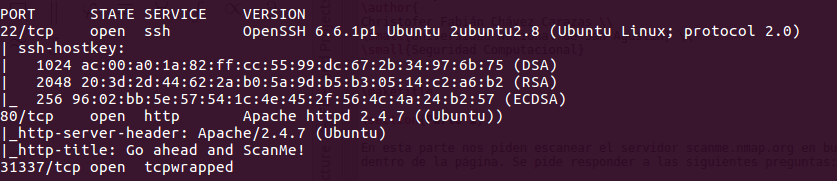
\includegraphics[scale = 0.5]{1.png}
 \end{figure}
 \item \textbf{Versión del SSH:} \\
  OpenSSH 6.6.1p1 Ubuntu 2ubuntu2.8 (Ubuntu Linux; protocol 2.0)
  \item \textbf{Versión del servidor:} \\
  Apache httpd 2.4.7
\end{enumerate}

\section{Parte 2}

En esta parte se nos pide hacer un monitoreo del tráfico del comando nmap con Wireshark. Se pide contestar las siguientes preguntas:

\begin{enumerate}
 \item \textbf{Que significa que un puerto esté cerrado:} \\
 \begin{figure}[H]
  \centering
  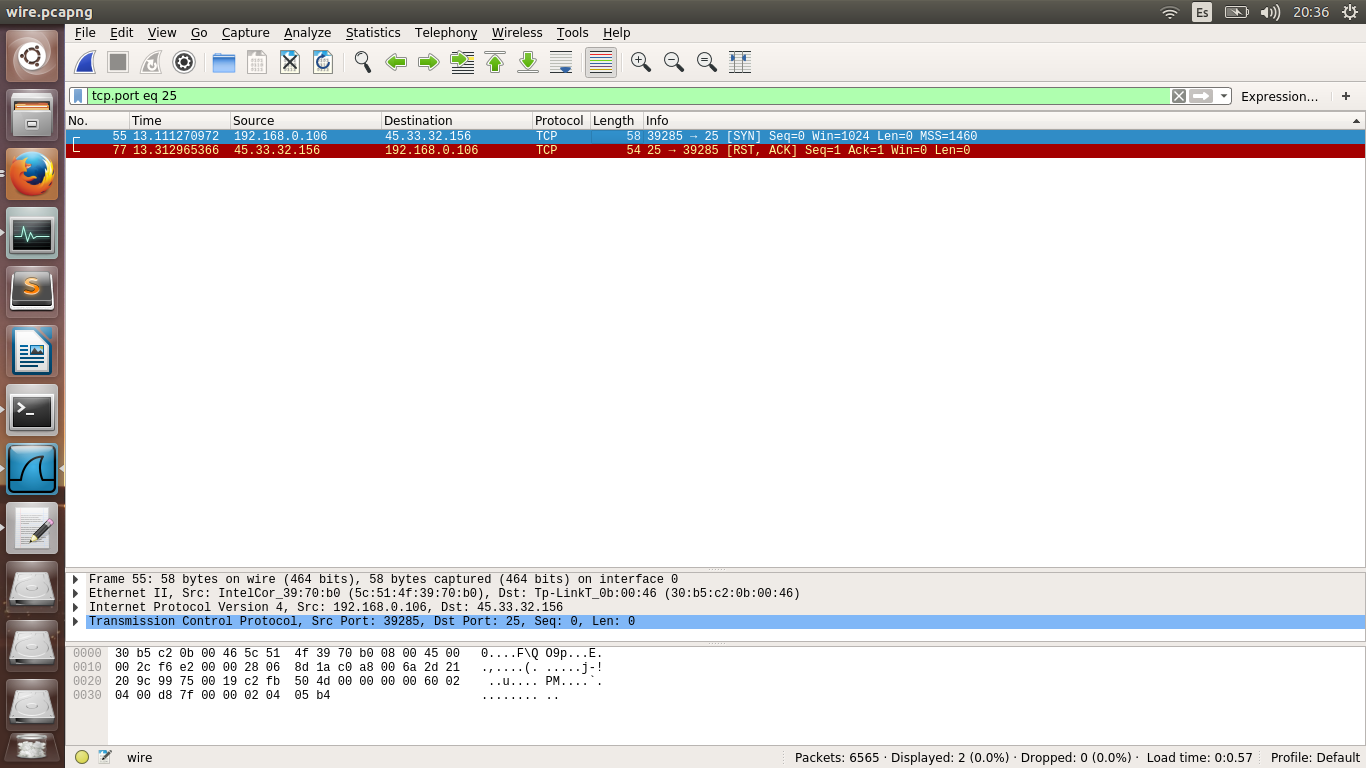
\includegraphics[scale = 0.3]{2.png}
 \end{figure}
 En la figura se muestra el paquete de envio y el paquete de retorno en color rojo. El paquete de retorno es del tipo
 [RST,ACK]
 \item \textbf{Que significa que un puerto esté filtrado:} \\
 \begin{figure}[H]
  \centering
  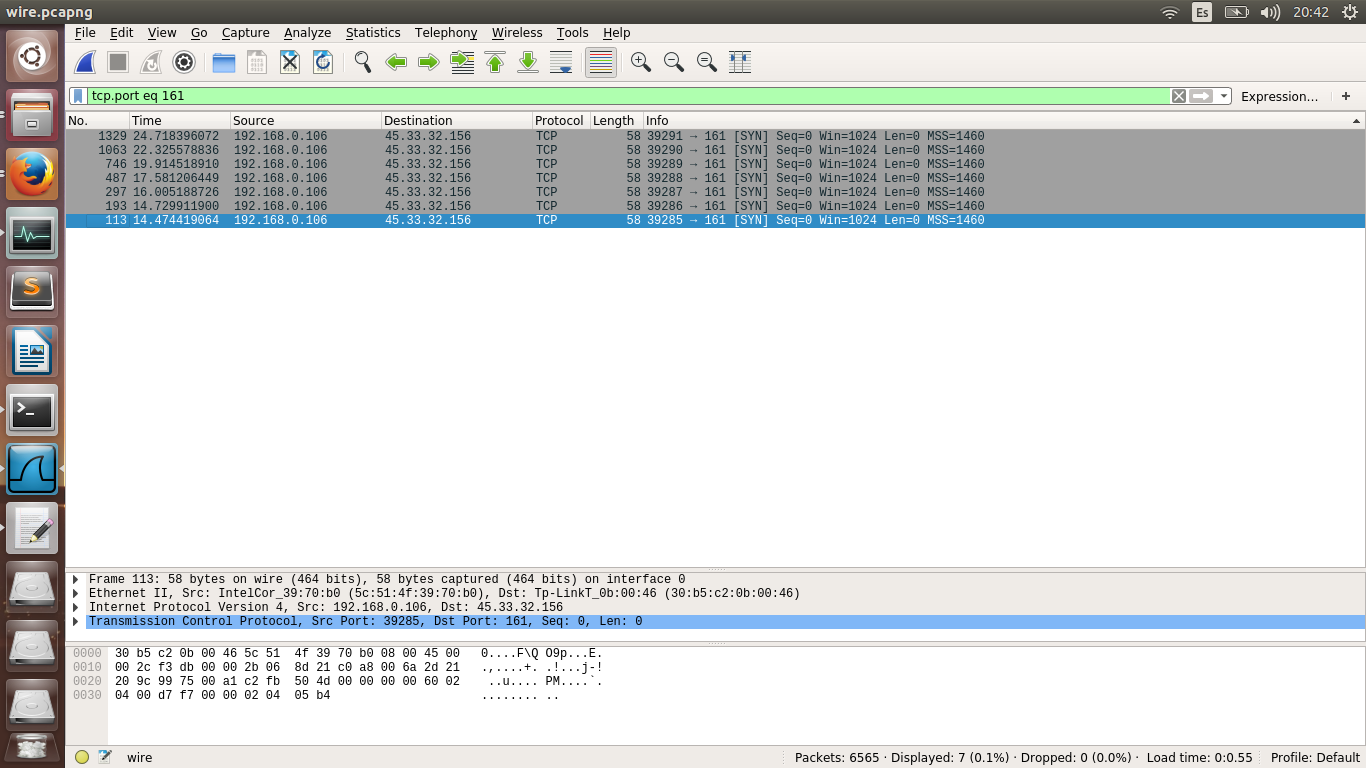
\includegraphics[scale = 0.3]{3.png}
 \end{figure}
 En la figura se muestran varios paquetes de envio, pero ninguno de regreso.
 \item \textbf{Además del HTTP GET, que otras peticiones http envía nmap:} \\
 \begin{figure}[H]
  \centering
  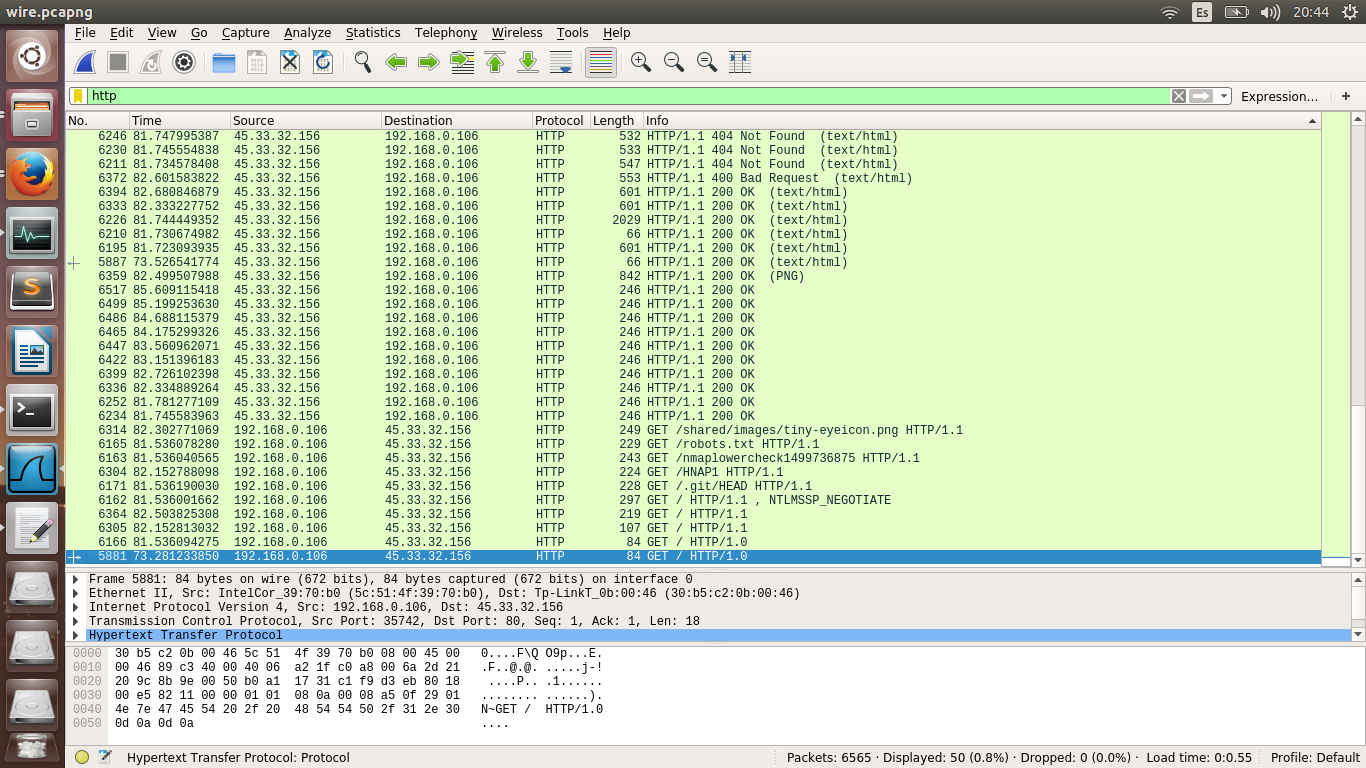
\includegraphics[scale = 0.3]{4.png}
 \end{figure}
  En la figura se muestra las peticiones GET
  \begin{figure}[H]
   \centering
   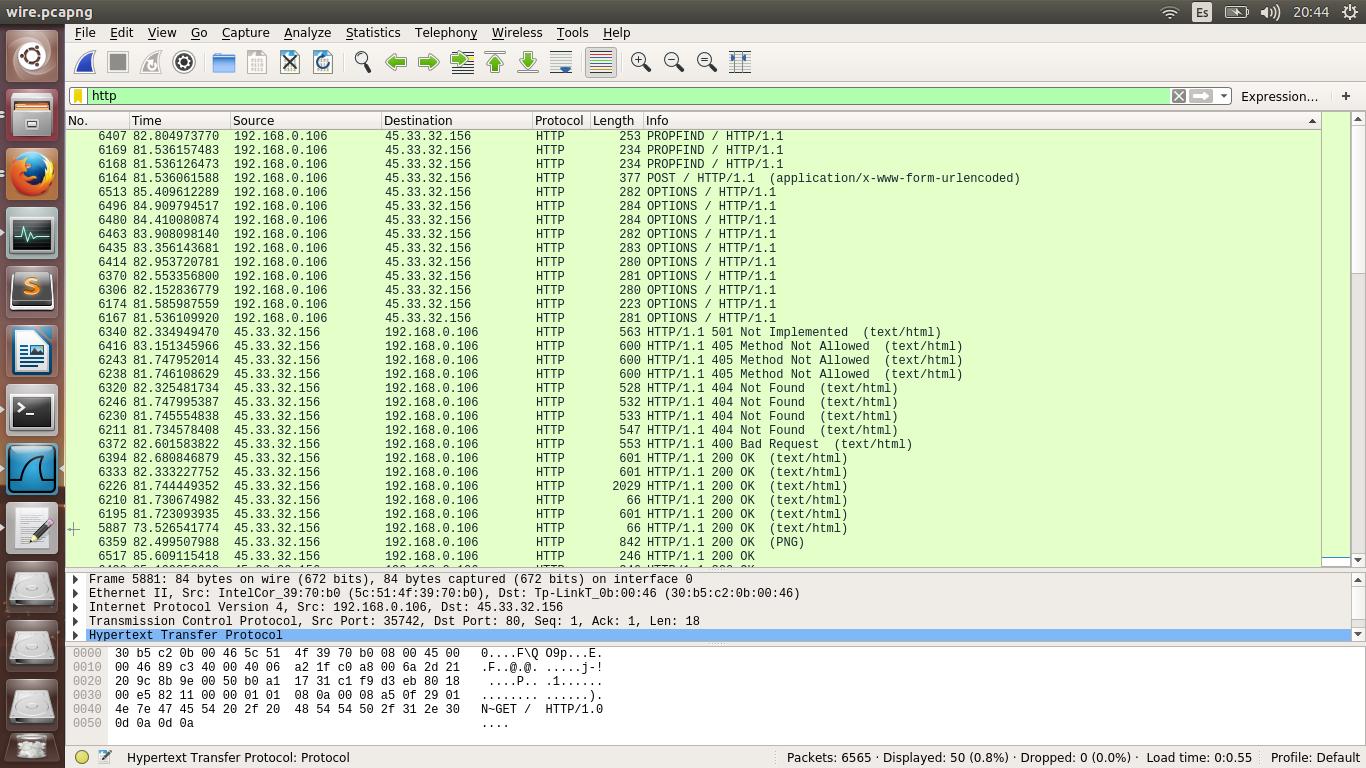
\includegraphics[scale = 0.3]{5.png}
  \end{figure}
  En la figura se muestra las peticiones PROPFIND, POST y OPTIONS.
\end{enumerate}

\section{Parte 3}

En esta parte se nos pide revisar un archivo con información de paquetes de una red. Se pide encontrar lo siguiente:
\begin{itemize}
 \item \textbf{5 direcciones IP de páginas web a las cuales haya entrado el dispositivo 10.30.22.101} \\
 grep '10.30.22.101.*80:' trace.txt \\
 23.74.61.15 \\
   184.25.56.67 \\
   74.125.239.103 \\
   66.235.138.194 \\
   17.178.96.59.80 \\
  \item \textbf{Encontrar la IP de destino y fuente de un escaneo de puertos, e indicar el rango} \\
  grep '[0-9]*\.[0-9]*\.[0-9]*\.[0-9]*\.161 $>$ ' trace.txt \\
  Destino: 10.30.5.234.161 \\
  Fuente: 10.30.1.65.55483 \\
  Rango: 1 - 65389 \\
  \item \textbf{Encontrar la IP de destino y fuente de un ataque DoS, e indicar cuántos paquetes han sido enviados} \\
  grep 'Flags [S].* length 0' trace.txt \\
  10.30.12.152 \\
  10.30.17.255 \\
  grep '10.30.12.152.[0-9]* $>$ 10.30.17.255.80: Flags [S].* length 0' trace.txt | wc -l \\
  26076 \\
\end{itemize}








\end{document}
